% !TEX root = ../../document.tex

\documentclass{subfiles}

\begin{document}

  \chapter{Algoritmo PageRank}
  \label{chap:pagerank}

    \section{Introducción}
    \label{sec:pagerank_intro}

      \paragraph{}
      El algoritmo \emph{PageRank} fue nombrado por primera vez en el trabajo \emph{The PageRank citation ranking: Bringing order to the web} \cite{page1999pagerank} publicado por \emph{Larry Page} y \emph{Sergey Brin}. La motivación del mismo fue tratar de realizar un \emph{ranking de importancia} (o relevancia) sobre los nodos de un \emph{grafo dirigido no ponderado} de tal manera que este esté basado únicamente en la estructura de dicho grafo.

      \paragraph{}
      La motivación de dicho trabajo fue la de tratar de mejorar el ranking de resultados del buscador de sitios web \emph{Google} en que estaban trabajando. Hasta la publicación de dicho trabajo, los sistemas de búsqueda se basaban en heurísticas como el número de ocurrencias de la palabra clave sobre la cual se basaba la búsqueda o el número de enlaces hacia dicha página.

      \paragraph{}
      Sin embargo, los rankings basados en este tipo de estrategias podían ser fácilmente manipulables con el fin de tratar de conseguir posicionarse en las primeras posiciones del sistema de búsqueda. Por ejemplo, una página web que se basara en la repetición de la misma palabra muchas veces, entonces aparecería en primer lugar en rankings basados en el número de ocurrencias para dicha palabra clave. En el caso de rankings basados en el número de enlac hacia dicha página, tampoco sería complejo manipular el resultado creando un número elevado de páginas web que contuvieran links hacia la página para la cual se pretende mejorar su posicionamiento.

      \paragraph{}
      La solución propuesta por \emph{Page} y \emph{Brin} para tratar de solucionar dicha problemática se basa en la generación de un ranking sobre los sitios web basado en la estructura del grafo subyacente, de tal manera que los vértices (sitios web) sobre los cuales existan aristas (enlaces) que provengan de otros vértices relevantes, tendrán una puntuación mayor que la de vértices que cuyo subconjunto de aristas los relacione con otros vértices menos relevantes.

      \paragraph{}
      La idea en que se basa el ranking se refiere por tanto a que los sitios web a los cuales se puede acceder a partir de otros sitios web considerados como importantes, entonces deberan encontrarse en primeras posiciones. Esta idea se extiende de manera inductiva sobre todos los vértices del grafo, puesto que tal y como veremos en las siguientes secciones converge hacia un estado estable (o \emph{distribución estacionaria} desde el punto de vista estadístico)

      \paragraph{}
      Para tratar de facilitar la comprensión acerca de esta idea a continuación se expone un ejemplo: Supongamos que en una red social como \emph{Twitter} (la cual se puede entender como un conjunto de usuarios que se relacionan entre si mediante relaciones de seguimiento, por lo que se puede ver como un grafo dirigido no poderado donde el conjunto de usuarios se refiere a los vértices y el conjunto de relaciones de seguimiento con las aristas) un usuario habitual (el cual no tiene un número elevado de seguidores) comienza a seguir a un antiguo amigo de la universidad, el cual tampoco tiene un gran número de seguidores.

      \paragraph{}
      La red social \emph{Twitter} envía una notificación a todos seguidores del usuario indicando que este ha empezado a seguir a su amigo de la universidad. Puesto que su número de seguidores es bajo dicha acción no tendrá una gran relevancia y muy probablemente nadie más comience a seguir al amigo de la universidad. Sin embargo, supongamos que nuestro usuario, en lugar de tener un conjunto reducido de seguidores, es una persona influyente en la red social, a la cual siguen millones de personas, entonces la notificación del nuevo seguimiento le llegará a muchos más usuarios y probablemente el amigo de la universidad verá como su número de seguidores aumenta notablemente.

      \paragraph{}
      A grandes rasgos, esta es la idea en que se basa el algoritmo \emph{PageRank}, es decir, la puntuación de un vértice del grafo se basa en la relevancia de los vértices que contienen aristas que apuntan hacia el propio vértice.

      \paragraph{}
      La idea inicial del algoritmo \emph{PageRank} era la de realizar un ranking basado en la estructura del grafo de la web (\emph{Web Graph}), sin embargo, tal y como se verá a lo largo del capítulo, los conceptos matemáticos en que se basa dicho ranking son extrapolables a cualquier entorno que se pueda representar a partir de una red o grafo. En el trabajo \emph{PageRank beyond the Web}\cite{gleich2015pagerank} \emph{Gleich} realiza un estudio acerca de los distintos entornos sobre los cuales se han aplicado estas ideas.

      \paragraph{}
      Entre otros, se han realizado trabajos sobre los cuales se ha aplicado el algoritmo \emph{PageRank} en áreas tan dispares como la Biología, para analizar las células más importantes a partir de las interrelaciones entre ellas. También se ha aplicado en el sector de la neurociencia por razones similares. En el caso de la literatura, se ha aplicado sobre el grafo generado a partir del sistema de citaciones de artículos de investigación. Otros ámbitos de aplicación han sido sistemas de planificación de tareas o incluso estudios acerca de resultados en deportes, para conocer los encuentros más relevantes.


      \paragraph{}
      [TODO hablar acerca de cómo se va a organizar el resto del capítulo]


    \section{Paseos Aleatorios}
    \label{sec:random_walks}

      \paragraph{}
      En esta sección se trata el concepto de \emph{Paseos Aleatorios}, el cual está intimamente relacionado con el algoritmo \emph{PageRank}. Para el desarrollo de esta sección se ha utilizado como herramienta bibliográfica el libro \emph{Randomized algorithms} \cite{motwani2010randomized} de \emph{Motwani} y \emph{Raghavan}, concretamente se ha prestado especial atención al \emph{capítulo 6: Markov Chains and Random Walks}. El resto de la sección se basará en la descripción de propiedades relacionadas con \emph{Paseos Aleatorios} para finalizar ilustrando la relacion de estos con \emph{PageRank}

      \paragraph{}
      Lo primero que haremos será describir en qué consiste un \emph{Paseo Aleatorio}. Para ello nos referiremos al grafo $G=(V,E)$ dirigido y no ponderado, el cual esta compuesto por $n = card(V)$ vértices y $m=card(E)$ aristas. Un paseo aleatorio se refiere entonces a un camino de longitud $l$ con origen en el vértice $v_{i_1}$ y final en $v_{i_l}$. Para que dicho camino constituya un paseo aleatorio, cada paso debe haber sido generado seleccionando de manera uniforme el siguiente vértice a visitar de entre los adyacentes al vértice actual. A continuación se describen las \emph{Cadenas de Markov} por su relación como herramienta de estudio para los paseos aleatorios.


      \subsection{Cadenas de Markov}
      \label{sec:markov_chains}

        \paragraph{}
        Para el estudio de paseos aleatorios, es apropiado utilizar la abstracción conocida como \emph{Cadenas de Markov}, las cuales están intimamente relacionadas con el concepto de grafo y máquina de estados. Una \emph{Cadena de Markov} $M$ se define como un proceso estocástico que consta de $n$ posibles estados, los cuales tienen asociadas un conjunto de probabilidades denotadas como $p_{ij}$ para indicar la probabilidad con la cual se pasará del estado $i$ al estado $j$.

        \paragraph{}
        Dichas probabilidades se pueden representar de manera matricial sobre una matriz de transiciones $P$ de tamaño $n*n$, de tal manera que la posición $(i,j)$ contenga el valor $p_{ij}$ construido tal y como se indica en el párrafo anterior. Notese por tanto, que $\sum_{j}p_{ij}=1$ para que la distribución de probabilidades sea válida, es decir, la suma de probabilidades para las transiciones sobre cada estado deben sumar $1$.

        \paragraph{}
        Supongase que se realiza un paseo aleatorio sobre la \emph{Cadena de Markov} $M$ cuya longitud $l$ es muy elevada ($l \gg n^2$), entonces, es fácil intuir que se visitará más de una vez cada estado. Sin embargo, el ratio de veces que se visitará cada estado muy probablemente no se distribuirá de manera uniforme, sino que habrá estados que serán visitados muchas más veces que otros. Esto depende en gran medida de la matriz de transicciones $P$. A la distribución de probabilidad generada sobre el ratio de visitas sobre cada nodo tras aplicar un paseo aleatorio de longitud elevada se le conoce como \emph{distribución estacionaria} y se denota como $\pi$.

        \begin{figure}
          \centering
          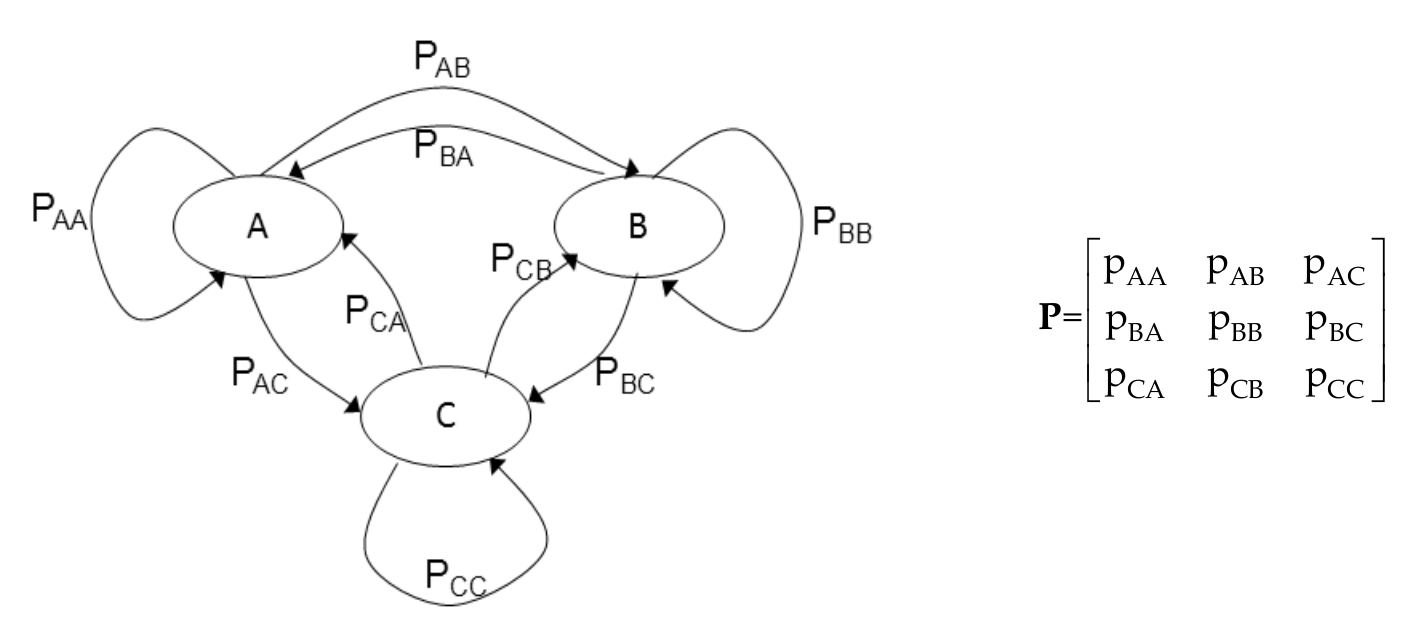
\includegraphics[width=0.6\textwidth]{markov-chain-example}
          \caption{Ejemplo de \emph{Cadena de Markov}. (Extraido de \cite{sanchez2012wireless})}
          \label{img:markov_chain_example}
        \end{figure}

        \paragraph{}
        En la figura \ref{img:markov_chain_example} (Extraido de \cite{sanchez2012wireless}) se muestra una cadena de markov constituida por 3 estados, tando en su forma de grafo dirigido como de forma matricial.

        \paragraph{}
        La distribución estacionaria $\pi$ existe siempre que la \emph{Cadena de Markov} $M$ permita que a partir de un determinado estado $i$, se pueda llegar al menos a otro estado $j$. La razón se debe a que si se llega al estado $i$ y este no contiene más posibles estados de salida, entonces el resto de épocas se seguirá en el mismo estado. A los estados que poseen esta característica se los denomina sumideros. La segunda restricción para que se pueda calcular la distrbución estacionaria $\pi$ es que la matriz de transiciones $P$ no debe ser periodica, es decir, no debe contener ciclos de probabilidad constante sobre los cuales el paseo aleatorio se quedaría iterando de manera indefinida.

        \paragraph{}
        Las definiciones descritas en este apartado se pueden extender de manera trivial al caso de grafos dirigidos sin más que utilizar cada vértice del grafo como un estado y construir la matriz $P$ de tal manera que $p_{ij}=\frac{A_{ij}}{d^-(i)}$ donde $d^-(i)$ representa el cardinal de aristas cuyo origen es el vértice $i$. Tal y como se verá posteriormente, el vector $\pi$ se corresponde con el resultado obtenido por el algoritmo \emph{PageRank} sobre una matriz $P$ de transicciones modificada.

      \subsection{Matriz Laplaciana de Paseos Aleatorios Normalizada}
      \label{sec:random_walk_normalized_laplacian_matrix}

        \paragraph{}
        En la sección \ref{sec:laplacian_matrix} se habló sobre la \emph{Matriz Laplacina}, la cual es una estrategia de representación, que ilustra distintas propiedades sobre el grafo subyacente. En este caso se describe una variación de la misma que es más apropiada para problemas relacionados con \emph{Paseos Aleatorios}. Esta se denota como $L^{{{\text{rw}}}}$ y se denomina \emph{Matriz Laplaciana de Paseos Aleatorios Normalizada}. La estrategia de construcción de la misma se indica en la ecuación \eqref{eq:random_walk_normalized_laplacian_matrix}. Esto consiste en asignar a la posición $(i,j)$ el opuesto de la probabilidad de transicción del vértice $i$ al vértice $j$. Además, en la diagonal $(i,i)$ se asigna el valor $1$ cuando el grado del vértice es mayor que $0$.

        \begin{equation}
        \label{eq:random_walk_normalized_laplacian_matrix}
          L_{{i,j}}^{{{\text{rw}}}}:={
          \begin{cases}
            1&{\mbox{if}}\ i=j\ {\mbox{and}}\ d(v_{i})\neq 0\\
            -{P_{ij}}&{\mbox{if}}\ i\neq j\ {\mbox{and}}\ v_{i}{\mbox{ is adjacent to }}v_{j}\\
            0&{\mbox{otherwise}}.
          \end{cases}}
        \end{equation}


      \paragraph{}
      Una vez descritos los \emph{Paseos Aleatorios}, junto con las \emph{Cadenas de Markov} y la \emph{Matriz Laplaciana de Paseos Aleatorios Normalizada}, ya se está en condiciones suficientes como para describir de manera formal el \emph{PageRank} de un determinado grafo, que se realizará en la siguiente sección. Para ello, se indicarán las dificultades que surgen sobre este problema en grafos reales, así como las soluciones utilizadas para poder hacer frente a estas.

    \section{Definición Formal}
    \label{sec:pagerank_formal_definition}

      \paragraph{}
      [TODO]

      \subsection{Teorema de Perron–Frobenius}
      \label{sec:perron_frobenius_theorem}

        \paragraph{}
        [TODO ]

    \section{Variantes}
    \label{sec:pagerank_variants}

      \paragraph{}
      [TODO ]

      \subsection{SymRank}
      \label{sec:symrank}

        \paragraph{}
        [TODO]

      \subsection{HITS}
      \label{sec:hits}

        \paragraph{}
        [TODO]

      \subsection{SALSA}
      \label{sec:salsa}

        \paragraph{}
        [TODO]

    \section{Algoritmo Básico}
    \label{sec:pagerank_algorithm}

      \paragraph{}
      [TODO ]

    \section{Soluciones Aproximadas}
    \label{sec:pagerank_algorithm_approximated}

      \paragraph{}
      [TODO ]

    \section{Conclusiones}
    \label{sec:pagerank_conclusions}

      \paragraph{}
      [TODO]

\end{document}
